Een harddisk\index{Harddisk} is een device waar data op opgeslagen kunnen worden. De data wordt op platen (Engels: Platters\index{Platter!Harddisk}), die voorzien zijn van een magnetische laag, weggeschreven. De platen draaien rond in een luchtdicht afgesloten behuizing met snelheden van 5400, 7200 of 10.000 rpm\index{RPM}\index{RPM!Harddisk} (rounds per minute). De platen zijn voorzien van fijne magnetische deeltjes. Een lees/schrijf-kop zet bij het schrijven de mini-magneetjes in een stand die overeen komen met een 1 of een 0. Bij het lezen leest de kop de stand van de magneetjes uit en weet zo of er een 1 of 0 staat. Voor elke plaat in de behuizing zijn er twee lees/schrijf-koppen. Een plaat kan aan twee kanten (Engels: Surfaces\index{Surface!Harddisk}) beschreven en uitgelezen worden, dus zowel de bovenkant als de onderkant van de plaat wordt gebruikt voor data opslag.

\begin{figure}
\includegraphics[width=0.5\textwidth]{Harddisk_intern.png}
\end{figure}

Data wordt in concentrische cirkels, tracks\index{Track}\index{Track!Harddisk}, weggeschreven. Een harddisk is een block-device en schrijft data dus weg in vaste blokken\index{Block}\index{Block!Harddisk}, bijvoorbeeld 512-bytes. Omdat er meerdere platen in een harddisk kunnen zitten en elke plaat 2 koppen heeft kan er dus data via verschillende koppen tegelijk gelezen en geschreven worden. Zo'n eenheid van data op dezelfde koppositie noemen we een cylinder. 

\begin{figure}
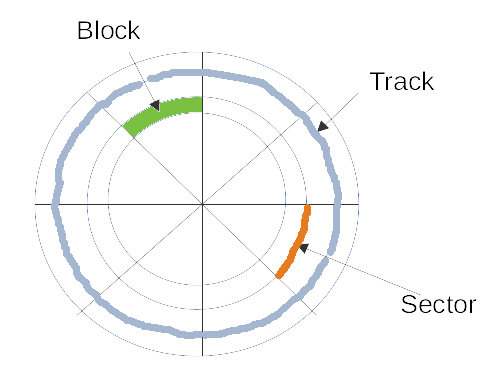
\includegraphics[width=0.5\textwidth]{HDD_Track-Sector-2.png}
\end{figure}

\begin{figure}
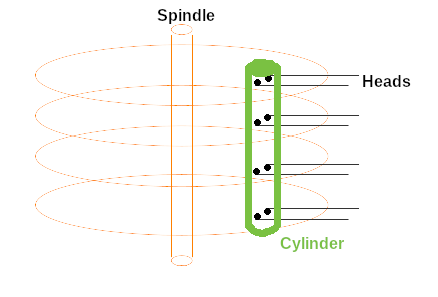
\includegraphics[width=0.5\textwidth]{HDD_Cylinder.png}
\end{figure}

De kop van een harddisk beweegt heen en weer tussen de draai-as (Spindle) en de rand van de platen. Deze beweging wordt gemaakt met een zogenaamde steppenmotor, die de kop in stappen verplaatst. De afstand die de kop heeft van de rand van de disk bepaalt de track waarop de kop zich bevindt. Het is de actuator\index{Actuator}\index{Actuator!Harddisk} die de kop verplaatst over de platen. De kop raakt de platen niet, er zit een klein stukje lucht tussen om te voorkomen dat de kop krassen op de surface maakt. Een track is verdeeld in sectoren\index{Sector}\index{Sector!Harddisk}. De sector is gelijk en synoniem aan de block grootte van de harddisk. Deze verdeling wordt gemaakt zodat bepaald kan worden waar data wordt weggeschreven (surface, track, sector).

Het verplaatsen van de head kost tijd en maakt een harddisk dus relatief traag. Door data tegelijk naar 1 cylinder te schrijven kunnen we de bewegingen van de kop minimaliseren en de data doorvoer maximaliseren.
